\section{Getting Started: Basic Examples}

The following sections demonstrate Dimple with four basic examples. The first example is a simple hidden Markov model. The second models a 4-bit XOR constraint. The third demonstrates how to use nested graphs. The final example is a simple LDPC code.  

\ifmatlab
See /demo/12\_Tutorial for the code.  
\fi

\ifjava
All java examples referenced in this section can be found in /solvers/java/src/main/java/com/analog/lyric/dimple/examples if Dimple has been installed from source.
\fi

\subsection{A Hidden Markov Model}

We consider a very simple hidden Markov model (HMM), the Rainy/Sunny HMM illustrated in the Wikipedia article about HMMs. Two friends who live far apart, Alice and Bob, have a daily phone conversation during which Bob mentions what he has been doing during the day. Alice knows that Bob's activity on a given day depends solely on the weather on that day, and knows some general trends about the evolution of weather in Bob's area.

Alice believes she can model the weather in Bob's area as a Markov chain with two states `Sunny' and `Rainy'. She remembers hearing that on the first day of last week it was quite likely (70\% chance) that it was sunny in Bob's town. She also knows that a sunny day follows another sunny day with 80\% chance, while a sunny day succeeds a rainy day with 50\% chance.

She knows Bob pretty well, and knows that Bob only ever does one of three things: stay inside to read a book, go for a walk, or cook. She knows that if it is sunny, Bob will go for a walk with 70\% probability, cook with 20\% probability, and stay inside with 10\% probability. Conversely, if it is rainy, Bob will go for a walk with 20\% probability, cook with 40\% probability, and stay inside with 40\% probability. 

Bob told Alice that he went for a walk on Monday, Tuesday, and Thursday, cooked on Wednesday and Friday, and read a book on Saturday and Sunday.

Alice wants to know what the most likely weather is for every day of last week. The above naturally defines an HMM which can easily be modeled within Dimple



\subsubsection*{Creating the Factor Graph}
The first thing to do in many Dimple programs, is to create a factor graph. This is easily done by instantiating a FactorGraph. 

\ifmatlab

See \/demo/12\_Tutorial/DimpleTutorial\_HMM.m

\fi

\ifjava

See solvers/java/src/main/java/com/analog/lyric/dimple/examples/HMM.java.

\fi


\ifmatlab

\begin{lstlisting}
HMM = FactorGraph();
\end{lstlisting}

\fi


\ifjava

\begin{lstlisting}
FactorGraph HMM = new FactorGraph();
\end{lstlisting}

\fi

\subsubsection*{Declaring Variables}
Once a Factor Graph has been defined, we can define the variables of the factor graph.  In our case, there will be seven variables, MondayWeather to SundayWeather. The syntax to create a variable is  \ifjava new \fi Discrete(domain,dimensions). In our case, the domain will consist of the two distinct values: Sunny and Rainy.\ifmatlab For now, we will not specify dimensions (this will be covered in 4 Bit XOR example). The domain should either be a cell, or a matrix of numbers.\fi

\ifmatlab

\begin{lstlisting}
Domain={'sunny','rainy'};
MondayWeather=Discrete(Domain);
TuesdayWeather=Discrete(Domain);
WednesdayWeather=Discrete(Domain);
ThursdayWeather=Discrete(Domain);
FridayWeather=Discrete(Domain);
SaturdayWeather=Discrete(Domain);
SundayWeather=Discrete(Domain);
\end{lstlisting}

IMPORTANT: In the above, had we used the declaration Domain=['sunny','rainy'] instead (square brackets instead of curly brackets), the domain would have consisted of 10 letters instead of 2 strings (i.e., the variables would have been 10-ary instead of binary).

\fi

\ifjava

\begin{lstlisting}
DiscreteDomain domain = DiscreteDomain.create("sunny", "rainy");
Discrete MondayWeather = new Discrete(domain);
Discrete TuesdayWeather = new Discrete(domain);
Discrete WednesdayWeather = new Discrete(domain);
Discrete ThursdayWeather = new Discrete(domain);
Discrete FridayWeather = new Discrete(domain);
Discrete SaturdayWeather = new Discrete(domain);
Discrete SundayWeather = new Discrete(domain);
\end{lstlisting}

\fi

\subsubsection*{Adding Factors}

We now add the different factors of the factor graph. We will first add the factors corresponding to the Markov Chain structure. This is done with addFactor, which is a method of the factor graph previously defined. 

\ifmatlab

The method has syntax addFactor(funchandle,arguments), where funchandle is the handle of a regular MATLAB function (which can be specified by the user), and the arguments are the variables involved in the factor being defined (in the same order as the inputs of the MATLAB function). The number of inputs of the function referred to by the function handle has to be equal to the number of arguments of addFactor.


In our case, we define a simple MC\_transition\_Tutorial(state1,state2) as follows (See /demos/12\_Tutorial/MC\_transition\_Tutorial.m):


\begin{lstlisting}
function [probability]=MC_transition_Tutorial(state1,state2)
 
switch state1
    case 'sunny'
        if state2=='sunny'
            probability=0.8;
        else
            probability=0.2;
            
        end
        
    case 'rainy'
        probability =0.5;
end 
\end{lstlisting}

\fi

\ifjava

The method has syntax addFactor(factorFunction,arguments), where factorFunction is an instance of a class that inherits from FactorFunction.  The arguments are the variables involved in the factor being defined (in the same order as the inputs of the real function of the Factor Function). The number of inputs of the function referred to by the function handle has to be equal to the number of arguments of addFactor.

In our case, we define a class called TransitionFactorFunction.

\begin{lstlisting}
	public static class TransitionFactorFunction extends FactorFunction
	{
		@Override
		public double eval(Object ... args)
		{
			String state1 = (String)args[0];
			String state2 = (String)args[1];
			
			if (state1.equals("sunny"))
			{
				if (state2.equals("sunny"))
				{
					return 0.8;
				}
				else
				{
					return 0.2;
				}
				
			}
			else
			{
				return 0.5;
			}
			
		}
	}
\end{lstlisting}

\fi

We can now add the factor to the factor graphs by using the addFactor method:

\ifmatlab

\begin{lstlisting}
HMM.addFactor(@MC_transition_Tutorial,MondayWeather,TuesdayWeather);
HMM.addFactor(@MC_transition_Tutorial,TuesdayWeather,WednesdayWeather);
HMM.addFactor(@MC_transition_Tutorial,WednesdayWeather,ThursdayWeather);
HMM.addFactor(@MC_transition_Tutorial,ThursdayWeather,FridayWeather);
HMM.addFactor(@MC_transition_Tutorial,FridayWeather,SaturdayWeather);
HMM.addFactor(@MC_transition_Tutorial,SaturdayWeather,SundayWeather);
\end{lstlisting}

\fi

\ifjava

\begin{lstlisting}
TransitionFactorFunction trans = new TransitionFactorFunction();
HMM.addFactor(trans, MondayWeather,TuesdayWeather);
HMM.addFactor(trans, TuesdayWeather,WednesdayWeather);
HMM.addFactor(trans, WednesdayWeather,ThursdayWeather);
HMM.addFactor(trans, ThursdayWeather,FridayWeather);
HMM.addFactor(trans, FridayWeather,SaturdayWeather);
HMM.addFactor(trans, SaturdayWeather,SundayWeather);
\end{lstlisting}

The java code first instantiates the factor function before connecting all of the variables.  It would be possible to create a new instance of the factor function for each addFactor call, but this would use unnecessary memory.

\fi

We now need to add factors corresponding to the observations of each day. As it happens, when using an addFactor method, the arguments need not be all random variables---some can be declared as constants. We see now how to use this fact to easily add the observations to each day. We first declare an observation function 

\ifmatlab

see /demo/12\_Tutorial/observation\_function\_Tutorial.m:


\begin{lstlisting}
function [probability]=observation_function_Tutorial(state,observation)
 
switch state    
    case 'sunny'
        
        switch observation
            
            case 'walk'
                probability=0.7;
            case 'book'
                probability=0.1;
            case 'cook'
                probability=0.2;
        end
        
    case 'rainy'
        
        switch observation
           
            case 'walk'
                probability=0.2;
            case 'book'
                probability=0.4;
            case 'cook'
                probability=0.4;
        end
end
\end{lstlisting}

\fi

\ifjava

see the ObservationFactorFunction from solvers/java/src/main/java/com/analog/lyric/dimple/examples/HMM.java.

\begin{lstlisting}
	public static class ObservationFactorFunction extends FactorFunction
	{
		@Override
		public double eval(Object ... args)
		{
			String state = (String)args[0];
			String observation = (String)args[1];
			
			if (state.equals("sunny"))
				if (observation.equals("walk"))
					return 0.7;
				else if (observation.equals("book"))
					return 0.1;
				else // cook
					return 0.2;
			else
				if (observation.equals("walk"))
					return 0.2;
				else if (observation.equals("book"))
					return 0.4;
				else // cook
					return 0.4;
		}
	}
\end{lstlisting}

\fi

Adding the observations is then very easy:

\ifmatlab
\begin{lstlisting}
HMM.addFactor(@observation_function_Tutorial,MondayWeather,'walk');
HMM.addFactor(@observation_function_Tutorial,TuesdayWeather,'walk');
HMM.addFactor(@observation_function_Tutorial,WednesdayWeather,'cook');
HMM.addFactor(@observation_function_Tutorial,ThursdayWeather,'walk');
HMM.addFactor(@observation_function_Tutorial,FridayWeather,'cook');
HMM.addFactor(@observation_function_Tutorial,SaturdayWeather,'book');
HMM.addFactor(@observation_function_Tutorial,SundayWeather,'book');
\end{lstlisting}
\fi

\ifjava

\begin{lstlisting}
ObservationFactorFunction obs = new ObservationFactorFunction();
HMM.addFactor(obs,MondayWeather,"walk");
HMM.addFactor(obs,TuesdayWeather,"walk");
HMM.addFactor(obs,WednesdayWeather,"cook");
HMM.addFactor(obs,ThursdayWeather,"walk");
HMM.addFactor(obs,FridayWeather,"cook");
HMM.addFactor(obs,SaturdayWeather,"book");
HMM.addFactor(obs,SundayWeather,"book");
\end{lstlisting}

\fi

As we can see, though the function itself depends on two variables, each factor only depends on one random variable (the other argument being set as a constant during the addFactor call). This in effect creates a factor connected only to one variable of the factor graph.

\ifmatlab

There is a cost incurred every time addFactor is called in MATLAB.  For large Factor Graphs with many factors of the same type, it can be advantageous to use the MATLAB vectorized version of addFactor.  The following code will create a transition factor between each pair of consecutive variables and will execute much more quickly than a for loop with addFactor.


\begin{lstlisting}
N = 1000;
Weather = Discrete(Domain,N,1);
HMM.addFactorVectorized(@MC_transition_Tutorial,Weather(1:(end-1)),Weather(2:end));
\end{lstlisting}

This works with continuous variables and Nested Graphs as well.  In addition, it's possible to specify which dimensions to vectorize over:


\begin{lstlisting}
N = 20;
b = Bit(3,N);
fg = FactorGraph();
fg.addFactorVectorized(@xorDelta,{b,2});
\end{lstlisting}

The previous code will create N xor factors across each of the N sets of 3 variables.

\fi

\subsubsection*{Specifying Inputs}


The last step consists in adding the prior for the MondayWeather variable. We could, as above, use a factor with a single variable. Let us introduce a new property to easily add a single variable factor--- the input property (on variables).  \ifjava When referring to "properties" in java, this implies there is a setter and getter so, in the case of inputs setInput and getInput. \fi

For a vector of probabilities (i.e., nonnegative numbers which sums up to one), \ifmatlab Variable.Input \fi \ifjava Variable.setInput \fi adds a single factor which depends on this variable only, with values equal to those given by the vector.

In our case, we do:

\ifmatlab

\begin{lstlisting}
MondayWeather.Input=[0.7 0.3];
\end{lstlisting}

\fi

\ifjava

\begin{lstlisting}
MondayWeather.setInput(0.7,0.3);
\end{lstlisting}

\fi

The Input property can be used in several different ways. Some notes of interest regarding the Input property:

\begin{itemize}
\item The Input method can typically be used for prior probabilities of the root variables in a Bayes Net, or for the initial node of a Markov Chain or HMM.
\item The Input property can also be used for any factors with only one variable, for instance, for observation factors (see the introduction to factor graphs on how to remove observations and turn them into single node factors).
\item The \ifmatlab observation\_function\_Tutorial \fi \ifjava ObservationFactorFunction \fi in the above example was not entirely required (see below)---we could have used the input property instead.
\item IMPORTANT: Unlike the addFactor method, the Input property can be used only once for each variable. That is, once you have specified an input for a variable, re-specifying this input will destroy the previous factor and create a new one. In the example above, using only the Input property, it would not have been possible to separately incorporate both the prior on Monday's weather and the factor corresponding to Monday�s observation. However, this feature is very useful when Input is used to specify external information, and when the user wants to see the effect of external information. Say for instance that Bob mentions to Alice that it rained on Wednesday. Alice can simply use the call \ifmatlab WednesdayWeather.Input=[0 1] \fi \ifjava WednesdayWeather.setInput(0,1)\fi. If Bob corrects himself and says he misremembered, and that it actually was sunny that day, Alice can correct the information using again the call \ifmatlab WednesdayWeather.Input=[1 0] \fi \ifjava WednesdayWeather.setInput(1,0)\fi.
\end{itemize}


\subsubsection*{Solving the Factor Graph}

Finally, we explain how to solve the factor graph by using the solve, iterate, and NumIterations factor graph methods.

The typical way of solving a factor graph will be by choosing the number of iterations and then running the solver for the desired number of iterations. In our case, this is simply done by typing the following code:

\ifmatlab

\begin{lstlisting}
HMM.NumIterations=20;
HMM.solve;
\end{lstlisting}

\fi

\ifjava

\begin{lstlisting}
HMM.getSolver().setNumIterations(20);
HMM.solve();
\end{lstlisting}

\fi

IMPORTANT:

By default, the solver will use either a Flooding Schedule or a Tree Schedule depending on whether the factor-graph contains cycles.  A loopy graph (one containing at least one cycle) will use a Flooding Schedule by default.  This schedule can be described as:

\begin{itemize}
\item Compute all variable nodes
\item Compute all factor nodes
\item Repeat for a specified number of iterations
\end{itemize}

If the factor-graph is a tree (one that contains no cycles), the solver will automatically detect this and use a Tree Schedule by default.  In this schedule, each node is updated in an order that will result in the correct beliefs being computed after just one iteration.  In this case, NumIterations should be 1, which is its default value.

\subsubsection*{Accessing Results}
Once the solver has finished running, we can access the marginal distribution of each variable by using the Belief property

\ifmatlab

\begin{lstlisting}
belief  = TuesdayWeather.Belief;
\end{lstlisting}

\fi

\ifjava

\begin{lstlisting}
double [] belief = TuesdayWeather.getBelief();
\end{lstlisting}

\fi

This returns a vector of probability of the same length as the domain total size (i.e., the product of its dimensions), with the probability of each domain variable.
Another way to solve the factor graph is to use the Solver.iterate(n) method, which runs the factor graph for n iterations (without arguments, it runs for 1 iteration).

\ifmatlab

\begin{lstlisting}
HMM.Solver.iterate();
HMM.Solver.iterate(5);
\end{lstlisting}

\fi

\ifjava

\begin{lstlisting}
HMM.getSolver().iterate();
HMM.getSolver().iterate(5);
\end{lstlisting}

\fi

IMPORTANT: The iterate method is useful to access intermediate results (i.e, see how beliefs change through the iterations).

IMPORTANT: One distinction between the solve and iterate methods is that all messages and beliefs are reinitialized when starting the solve method. Running solve twice in a row is therefore identical to running it once, unlike iterate.  When calling iterate() for the first time, first call initialize(), which reinitialize all messages.


\subsection{A 4-bit XOR}

The following example creates a simple factor graph with 4 variables tied through a 4-bit XOR, with `priors' (we abuse language here and call `prior' the probability distribution of each random variable if they were not tied through the 4-bit XOR).

Through this example, we will learn how to define arrays of random variables, see how to use MATLAB indexing within Dimple, see an example of a hard constraint in a factor graph, and see how to use the Bit type of random variable.

We consider a set of four random variables (B1,B2,B3,B4) taking values 0 or 1. The joint probability distribution is given by:


\[
 Pr(B_1,B_2,B_3,B_4) = \delta_{B_1+B_2+B_3+B_4=0(mod2)}  P(B_1)P(B_2)P(B_3)P(B_4)  
\]


where the delta function   is equal to 1 if the underlying constraint is 
satisfied, and 0 otherwise (this ensures that illegal assignment have 
probability zero). The $P(B_i)$ are single variable factors which help model 
which values of $ B_i $  are more likely to be taken (we call them `priors', 
though, once again, this is an abuse of language. Typically, the factor
 will represent an observation of  $ O_i $ of variable  $ B_i $, and the factor 
$ P(B_i) $  is 
set equal to the normalized function  $ P(O_i | B_i ) $ \footnote { Normalizing $ P(O_i|B_i) $ happens to be equal to $P(B_i|O_i)$ in a
factor graph with only the two variables $O_i$ and $B_i$ with a prior on both values of 
$B_i$ being equally likely. }



For our example, we will choose  $P(B_1 =1)=P(B_2=1)=P(B_3=1)=.8$ and  
$P(B_4=1)$ = 0.5.

We will build our factor graph in two different ways. The first directly uses a 4-bit XOR, and uses mostly tools seen in the previous example, while the second introduces the Bit kind of random variable, and how to use an intermediate variable to reduce the degree of a factor graph with parity checks (i.e., XOR function).

The first way of building the factor graph uses an inefficient N-bit XOR function defined as follows 

\ifmatlab

From /demo/12\_Tutorial/BadNBitXorDelta\_Tutorial.m:

\begin{lstlisting}
function [valid]=BadNBitXorDelta_Tutorial(variables)
 
valid=mod(sum(variables),2)==0;

end
\end{lstlisting}

\fi

\ifjava


See solvers/java/src/main/java/com/analog/lyric/dimple/examples/BadNBitXor.java

\begin{lstlisting}
	public static class BadNBitXorFactor extends FactorFunction
	{
		@Override
		public double eval(Object ... args)
		{
			int sum = 0;
			for (int i = 0; i < args.length; i++)
				sum += (Integer)args[i];
			
			return (sum % 2) == 0 ? 1 : 0;
		}
	}
\end{lstlisting}

\fi

Using everything we have learned in the previous example, the sequence of instructions we use is simply 

\ifmatlab 

From /demo/12\_Tutorial/DimpleTutorial\_BadNBitXor.m:


\begin{lstlisting}
FourBitXor=FactorGraph();
Domain=[0;1];
B1=Discrete(Domain);
B2=Discrete(Domain);
B3=Discrete(Domain);
B4=Discrete(Domain);
FourBitXor.addFactor(@BadNBitXorDelta_Tutorial, [B1,B2,B3,B4]);
B1.Input=[0.2 0.8];
B2.Input=[0.2 0.8];
B3.Input=[0.2 0.8];
B4.Input=[0.5 0.5];
FourBitXor.solve;
disp(B1.Value);
disp(B1.Belief);
\end{lstlisting}

Note that the MATLAB BadNBitXorDelta\_Tutorial is a function which takes only ONE argument, but this argument is an array. This is reflected in the declaration FourBitXor.addFactor (@BadNBitXorDelta\_Tutorial, [B1,B2,B3,B4]), where we created an array of random variables using square brackets.

\fi

\ifjava

\begin{lstlisting}
FactorGraph fourBitXor = new FactorGraph();
DiscreteDomain domain = DiscreteDomain.bit();
Discrete b1 = new Discrete(domain);
Discrete b2 = new Discrete(domain);
Discrete b3 = new Discrete(domain);
Discrete b4 = new Discrete(domain);
fourBitXor.addFactor(new BadNBitXorFactor(),b1,b2,b3,b4);
b1.setInput(0.2,0.8);
b2.setInput(0.2,0.8);
b3.setInput(0.2,0.8);
b4.setInput(0.5,0.5);
fourBitXor.solve();
System.out.println(b4.getValue());
System.out.println(Arrays.toString(b4.getBelief()));
\end{lstlisting}

\fi


IMPORTANT: We also introduce the Discrete method `Value', which returns the most likely assignment of that random variable.

\ifmatlab

The first remark above is rather important, as it highlights of the concept of arrays of random variables in the MATLAB Dimple API.  Dimple handles arrays of random variables in a very natural manner, and most array indexing operations of MATLAB are supported in Dimple in a similar fashion. 

To create a multidimensional array of random variables in the MATLAB Dimple API, we construct a Variable class instance where every constructor argument after the first is a dimension of an array:

\begin{lstlisting}
VarArray=Variable(Domain,dimension1,dimension2,.., dimensionk) 
\end{lstlisting}

creates an array of variables with domain `Domain', and with dimensions [dimension1][dimension2]..[ dimensionk]. 

IMPORTANT: If only one dimension is specified, Dimple creates a square array.


\begin{lstlisting}
VarArray1=Discrete(Domain,3,1)
VarArray2=Discrete(Domain,3)
VarArray3=Discrete(Domain,3,3)
\end{lstlisting}



In the example above, VarArray1 is a vector of 3 random variables with domain Domain, while VarArray2 and VarArray2 are both a 3-by-3 matrix of random variables with domain Domain.

Another way to create an array is, as above, to group the variables using square brackets:


\begin{lstlisting}
RowArray=[ B1 B2 B3 B4];
ColumnArray=RowArray';
\end{lstlisting}

IMPORTANT: The above method is a simple "grouping" (reference) of variables  ; it does not duplicate them.

Concatenation and subindexing of random arrays work in exactly the same fashion as MATLAB.


\begin{lstlisting}
SubArray1=VarArray2(2,1:2);
SubArray2=VarArray2(1,2:3);
SubArray3=[SubArray1;SubArray2];
\end{lstlisting}

repmat works as well.  The following code snippet will set C to a 10x10 Bit matrix.  Rather than creating new
variables, it simply replicates the existing variables.  

\begin{lstlisting}
b = Bit(10,1);
c = repmat(b,1,10);
\end{lstlisting}



Using the Variable methods Belief, Value or Domain on a random array returns the array of Beliefs (resp. ML values, domains, etc..) for these variables.


\begin{lstlisting}
SubArray2.Value
\end{lstlisting}

returns a (1,2) array containing the most likely values of VarArray2(1,2) and VarArray2(1,3).

IMPORTANT: Since Beliefs or Inputs are arrays themselves, calling them on an array returns an array one dimension larger.

\fi

Often, we will find it useful to have random Bits. For that purpose, one can directly create random Bits with the Bit class. A Bit is simply a Discrete with Domain [0, 1]. Also, in order to simplify Input declarations, for a Bit variable named BitVar, BitVar.Input takes a single number, the probability of 1. 

\ifmatlab
Similarly, BitVar.Belief returns the marginal probability of BitVar being equal to 1.
\fi

The second version of the 4-bit XOR will uses Bit variables to represent our random variables. Furthermore, it will decompose the 4 bits XOR into two 3-bits XOR. It is indeed easy to prove that $ B_1 + B_2 + B_3 + B_4 = 0(mod 2) $ is equivalent to


\begin{eqnarray*}
B_1+B_2+C &=& 0(mod 2) \\
B_3+B_4+C &=& 0(mod 2)
\end{eqnarray*}


for an internal bit C. While the reduction from one 4-bit to two 3-bit XORs might not seem tremendous, it is easy to see that more generally, any N-bit XOR can be reduced to a tree of 3-bit XORs, with depth log(N). Because the complexity of running Belief Propagation is exponential in the degree of factors, using this technique leads to dramatic speed improvements.

Using all the techniques mentioned above, we derive a new factor graph for the 4-bit XOR, equivalent to the one previously defined 

\ifmatlab

From /demo/12\_Tutorial/xorDeltaTutorial.m:


\begin{lstlisting}
function valid = XorDeltaTutorial(x,y,z)       
    valid = bitXor(bitXor(x,y),z) == 0;
end
\end{lstlisting}



From demo/12\_Tutorial/DimpleTutorial\_4BitXor.m:

\begin{lstlisting}
XorGraph = FactorGraph();
b = Bit(4,1);
c = Bit();
XorGraph.addFactor(@XorDeltaTutorial,b(1),b(2),c);
XorGraph.addFactor(@XorDeltaTutorial,b(3),b(4),c);
b.Input = [ .8 .8 .8 .5];
XorGraph.solve();
disp(b.Belief);
disp(b.Value);
\end{lstlisting}

\fi

\ifjava

From solvers/java/src/main/java/com/analog/lyric/dimple/examples/ThreeBitXor.java

\begin{lstlisting}
public class ThreeBitXor extends FactorFunction
{
	@Override
	public double eval(Object ... args)
	{
		int arg0 = (Integer)args[0];
		int arg1 = (Integer)args[1];
		int arg2 = (Integer)args[2];
		
		return (arg0 ^ arg1 ^ arg2) == 0 ? 1 : 0;
	}
}
\end{lstlisting}

From solvers/java/src/main/java/com/analog/lyric/dimple/examples/FourBitXor.java

\begin{lstlisting}

	FactorGraph xorGraph = new FactorGraph();
	Bit [] b = new Bit[4];
	for (int i = 0; i < b.length; i++)
		b[i] = new Bit();
	Bit c = new Bit();
		
	ThreeBitXor xd = new ThreeBitXor();
		
	xorGraph.addFactor(xd,b[0],b[1],c); 
	xorGraph.addFactor(xd,b[2],b[3],c);
		
	double [] inputs = new double [] {.8, .8, .8, .5};
	for (int i = 0; i < inputs.length; i++)
		b[i].setInput(inputs[i]);
		
	xorGraph.solve();
		
	for (int i = 0; i < b.length; i++)
		System.out.println(b[i].getP1());
	for (int i = 0; i < b.length; i++)
		System.out.println(b[i].getValue());

\end{lstlisting}

\fi

The following figure represents the Factor Graph that is created and solved in this example.

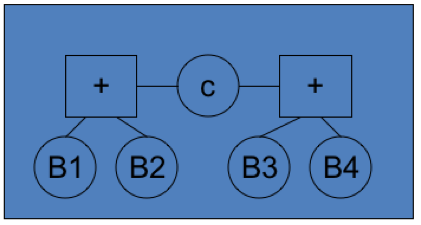
\includegraphics{images/FactorGraphTemplate.png}

\subsection{Nested Graphs}
\label{sec:nestedGraphs}
Suppose we wish to use two 4-bit XORs from the previous example to create a 6-bit code.  The following diagram shows our desired Factor Graph.

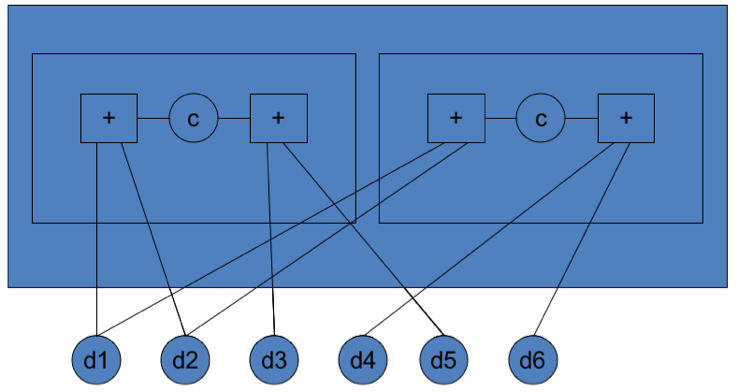
\includegraphics{images/NestedGraph.png}

Dimple provides a way to replicate multiple copies of a Factor Graph and nest these instances in a containing Factor Graph. A nested Factor Graph can be seen as a special factor function between a set of variables (`connector variables'), which, when `zoomed in,' is in fact another factor graph, with factors involving both the connector variables, and other `internal variables.' In the second version of the XOR example, we created a 4-bit XOR connected to 4 variables, by also creating an extra Bit C. What if we wanted to use that construction as a 4-bit XOR for potentially many different sets of 4 bits, overlapping or not, by replicating the factor graph as needed? Nested factor graphs provide an elegant solution to this problem.

A nestable factor graph is created by specifying first a set  of "connector" random variables, and instantiating a FactorGraph with these variables passed in to the constructor.

IMPORTANT: The factor graph defined this way is still a proper factor graph, and in principle, we can run BP on it. However, in practice, it is used as a "helper" factor graph (and   are "helper" random variables), which will mostly be replicated in the actual factor graph of interest.

The following code creates a nestable factor graph, with connector variables $ (B_1,B_2,B_3,B_4) $

\ifmatlab

From /demo/12\_Tutorial/DimpleTutorialNested.m:


\begin{lstlisting}
% Define 4 bit Xor from two 3 bit Xors
%%%%%%%%%%%%%%%%%%%%%%%%%%%%%%%%%%%%%%
b = Bit(4,1);
XorGraph = FactorGraph(b);
c = Bit();
XorGraph.addFactor(@XorDeltaTutorial,b(1),b(2),c);
XorGraph.addFactor(@XorDeltaTutorial,b(3),b(4),c);
\end{lstlisting}

\fi

\ifjava

See solvers/java/src/main/java/com/analog/lyric/dimple/examples/Nested.java

\begin{lstlisting}
////////////////////////////////////// 
// Define 4 bit xor from two 3 bit xors 
////////////////////////////////////// 
Bit [] b = new Bit[4];
for (int i = 0; i < b.length; i++)
	b[i] = new Bit();
		
FactorGraph xorGraph = new FactorGraph(b);
		
Bit c = new Bit(); 
ThreeBitXor xd = new ThreeBitXor();
		
xorGraph.addFactor(xd,b[0],b[1],c); 
xorGraph.addFactor(xd,b[2],b[3],c);
\end{lstlisting}
\fi

IMPORTANT: In principle, variables attached to a Factor Graph can be defined before or after defining the factor graph (but obviously always before the factors they are connected to). However, connector variables naturally need to be defined before the nestable factor graph.

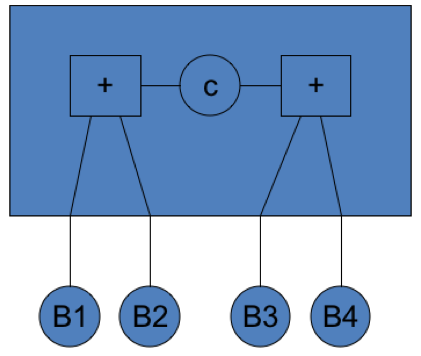
\includegraphics{images/BoundaryVariables.png}

Consider a nestable factor graph NestableFactorGraph(connectvar1, connectvar2,..,vark) with k connector variables. Consider also an actual factor graph of interest, FactorGraph, containing (among others) k variables of interest (var1,..,vark). By using the addGraph method, we can replicate the NestableFactorGraph and use it to connect the variables (var1,..,vark) in the same way the connector variables are connected in the nestable factor graph. The method is: FactorGraph.addGraph(NestableFactorGraph,var1,..,vark).

In essence, the nestable factor graph represents a factor between the dummy connector variables, and the addGraph method is adding the factor to the desired actual variables.

IMPORTANT: Nested factor graphs support arbitrary levels of nesting.  That is, a nested factor graph can be composed of nested factor graphs.

Armed with this tool, we can very simply use our custom 4-bit XOR to implement the factor graph described at the beginning of the section:

\ifmatlab

\begin{lstlisting}
%%%%%%%%%%%%%%%%%%%%%%%%%%%%%%%%%%%%%%
% Create graph for 6 bit code
%%%%%%%%%%%%%%%%%%%%%%%%%%%%%%%%%%%%%%    


d = Bit(6,1);
MyGraph = FactorGraph(d);
MyGraph.addGraph(XorGraph,d([1:3 5]));
MyGraph.addGraph(XorGraph,d([1 2 4 6]));

%%%%%%%%%%%%%%%%%%%%%%%%%%%%%%%%%%%%%%
% Set input and Solve
%%%%%%%%%%%%%%%%%%%%%%%%%%%%%%%%%%%%%%

d.Input = [.75 .6 .9 .1 .2 .9];
MyGraph.NumIterations = 20;
MyGraph.solve();
disp(d.Value');
\end{lstlisting}



IMPORTANT: Note the use of standard MATLAB array indexing in the d([1:3 5]) method above. Also, note that technically, our nestable factor graph declared above only had one argument (not four), an array of four random variables (as opposed to four separately declared random variables). As a result, the addGraph call requires a single argument---an array of four random 

\fi

\ifjava
\begin{lstlisting}
////////////////////////////////////// 
// Create graph for 6 bit code 
////////////////////////////////////// 
Bit [] d = new Bit[6];
for (int i = 0; i < d.length; i++)
	d[i] = new Bit();

FactorGraph myGraph = new FactorGraph(d); 
myGraph.addFactor(xorGraph,d[0],d[1],d[2],d[4]); 
myGraph.addFactor(xorGraph,d[0],d[1],d[3],d[5]);
////////////////////////////////////// 
// Set input and Solve 
////////////////////////////////////// 
double [] inputs = new double [] {.75, .6, .9, .1, .2, .9};
for (int i = 0; i < inputs.length; i++)
	d[i].setInput(inputs[i]);
myGraph.solve();
for (int i = 0; i < d.length; i++)
	System.out.println(d[i].getValue());
\end{lstlisting}
\fi

\ifmatlab

\subsection{An LDPC Code}
For our last example, we will show how to use a library function to very quickly code up a complex factor graph.

We present the code that defines a Factor Graph to decode an LDPC (low-density parity check) code (in the file /demo/11\_SingleCodewordLDPC/createLDPC.m):

\begin{lstlisting}
function [ldpc,x] = createLdpc()
    A = load('matrixout.txt');
    blockLength = size(A,2);
    numCheckEquations = size(A,1);
    ldpc = FactorGraph();   
        x = Bit(blockLength,1);     
        for i = 1:numCheckEquations
            varIndices = find(A(i,:));
            gd = getNBitXorDef(length(varIndices));
            ldpc.addGraph(gd,x(varIndices));
        end       
     ldpc.NumIterations = 100;
end
\end{lstlisting}


At this point, all the code above should be clear, except for the getNBitXorDef call. getNBitXorDef(N) returns a nestable factor graph with an array of N bits as connected variables, representing an N-bit XOR factor between those N bits. It implements the most efficient (in some sense) implementation of an N-bit XOR using a tree of 3-bits XORs.

The check matrix connectivity is loaded from a file into matrix A. The for loop iterates all check equations, creates a nestable n-bit XOR Graph and adds that graph to the LDPC.  The user can set Input on x and the returned variables, solve the ldpc object, and retrieve the results with Value or Beliefs.

\fi
